%!Tex Ts-program = lualatex
%!figpath = .
\documentclass[11pt,openany]{book}              % Book class in 11 points
\usepackage{luacode}
%\documentclass[justified,twoside]{tufte-book}
%\usepackage[UTF8]{ctex}
%\usepackage[english]{babel}


\parindent0pt  \parskip10pt             % make block paragraphs
%\raggedright                            % do not right justify
\usepackage{xcolor}
\usepackage{float}
\usepackage{amsmath}
\usepackage{amssymb}
\usepackage{bm}
\usepackage[round]{natbib}
\usepackage{graphicx}
\usepackage{animate}
\usepackage{matlab-prettifier}
\usepackage{subfigure}
\usepackage{amsthm}
\usepackage{tgpagella}
\usepackage{enumerate}
\usepackage{emptypage}
\usepackage{multirow}
\usepackage{booktabs}
\usepackage{braket}
\usepackage[LGR,T1]{fontenc}
\newcommand{\textgreek}[1]{\begingroup\fontencoding{LGR}\selectfont#1\endgroup}
\usepackage{lipsum}
\usepackage{tcolorbox}


\usepackage{microtype}


\definecolor{echodrk}{HTML}{0099cc}
\definecolor{mymauve}{rgb}{0.58,0,0.82}
\usepackage[colorlinks,linkcolor=mymauve,citecolor=echodrk]{hyperref}
\usepackage{cleveref}
\usepackage{pgfplots}

\definecolor{boxgray}{rgb}{0.9,0.9,0.9}
\definecolor{boxpink}{rgb}{0.9,0.7,0.7}

\renewcommand\vec{\mathbf}
\newcommand\mat{\mathbf}

\makeatletter
\renewcommand{\thesection}{%
  \ifnum\c@chapter<1 \@arabic\c@section
  \else \thechapter.\@arabic\c@section
  \fi
}
\makeatother



\usepackage{marginnote}
\renewcommand*{\marginfont}{\footnotesize}
\newcommand{\joan}[1]{{\color{green}#1}}
\newcommand{\michael}[1]{{\color{magenta}#1}} \newcommand{\taco}[1]{{\color{blue}#1}}
\newcommand{\petar}[1]{{\color{cyan}#1}}


\definecolor{olivegreen}{HTML}{006400}
\definecolor{echoblue}{HTML}{0099CC}
\definecolor{gold}{HTML}{F09A00}
\definecolor{vividred}{HTML}{E60B42}
\definecolor{echonavy}{HTML}{0054B2}
\definecolor{darkgry}{HTML}{333333}
\definecolor{echopurple}{HTML}{9400D1}
\usepackage{tikz}
\tikzset{every picture/.style={line width=0.75pt}} %set default line width to 0.75pt    


\newcommand*{\horzbar}{\rule[.5ex]{2.5ex}{0.5pt}}
\newtheoremstyle{break}%
{\topsep}{\topsep}%
{\itshape}{}%
{\bfseries}{}%
{\newline}{}%
%\theoremstyle{break}

\newtheorem{definition}{Definition}
\newtheorem{theorem}{Theorem}
\newtheorem{remark}{Remark}
\newtheorem{example}{Example}
\newtheorem{corollary}{Corollary}
\newtheorem{consequence}{Consequence}
\newtheorem{conjecture}{Conjecture}
\newtheorem{problem}{Problem}
\newtheorem{solution}{Solution}
\newcommand{\sign}{{\rm sign}}
\newcommand{\argmin}{\mathop{\rm argmin}}
\newcommand{\argmax}{\mathop{\rm argmax}}
\newcommand{\tr}{\mathop{\rm tr}}
\newcommand{\dd}{{\rm d}}

\usepackage{fancyhdr}

\fancypagestyle{plain}{ %
  \fancyhf{} % remove everything
  \renewcommand{\headrulewidth}{0pt} % remove lines as well
  \renewcommand{\footrulewidth}{0pt}
}


\fancypagestyle{fancybook}{%
  \fancyhf{}%
  % Note the ## here. It's required because \fancypagestyle is making a macro (\ps@fancybook).
  % If we just wrote #1, TeX would think that it's the argument to \ps@fancybook, but
  % \ps@fancybook doesn't take any arguments, so TeX would complain with an error message.
  % You are not expected to understand this.
  \renewcommand*{\sectionmark}[1]{ \markright{\thesection\ ##1} }%
  %\renewcommand*{\chaptermark}[1]{ \markboth{\chaptername\ \thechapter: ##1}{} }%
  % Increase the length of the header such that the folios 
  % (typography jargon for page numbers) move into the margin
  \fancyhfoffset[LE]{6mm}% slightly less than 0.25in
  \fancyhfoffset[RO]{6mm}%
  % Put some space and a vertical bar between the folio and the rest of the header
  \fancyhead[LE]{\thepage\hskip3mm\vrule\hskip3mm}%
  \fancyhead[RO]{\rightmark\hskip3mm\vrule\hskip3mm\thepage}%
}
\pagestyle{fancybook}

%\usepackage{appendix}

\usepackage[titletoc]{appendix}


%\fancyhf[HLE,HRO]{Bruna et al.}
\pagestyle{empty}

\newcommand{\rarr}{\rightarrow}

\begin{document}
\chapter*{Some Property of Ising Model}
\vspace{-1cm}
{\fontsize{18.0pt}{\baselineskip}\selectfont  Yongle Bai 202011150087}

\section{The detailed setup of the problem}
The Ising model (or Lenz-Ising model or Ising-Lenz model), named after the physicists Ernst Ising and Wilhelm Lenz, is a mathematical model of ferromagnetism in statistical mechanics.
The model consists of discrete variables that represent magnetic dipole moments of atomic "spins" that can be in one of two states (+1 or −1).
The spins are arranged in a graph, usually a lattice (where the local structure repeats periodically in all directions), allowing each spin to interact with its neighbors.
Neighboring spins that agree have a lower energy than those that disagree; the system tends to the lowest energy but heat disturbs this tendency, thus creating the possibility of different structural phases.
The model allows the identification of phase transitions as a simplified model of reality.
The two-dimensional square-lattice Ising model is one of the simplest statistical models to show a phase transition.

Now we consider a \(2\)-dimensional lattice with period boundary and size \(n \times n\).
We use \(\Lambda:=\mathbb{Z}_n \times \mathbb{Z}_n\) as the index set.
Let \(\sigma=\{ \sigma_k\}_{k \in \Lambda}\) be the state of the lattice.
The direction of each spin in the lattice is regarded as an element in \(\sigma\), and \(\pm 1\) represent two direction.
For any two adjacent sites \(i,j\in \Lambda \) there is a spin-spin interaction \(J\).
Also, a site \(j\in \Lambda \) has an external magnetic field \(H\) interacting with it. The energy of a configuration \(\sigma\) is given by the Hamiltonian function
\begin{equation}\label{equ:1}
	H(\sigma)=-\sum_{i,j\in\Lambda,i \sim j} J \sigma_i \sigma_j-\sum_{i \in \Lambda}H \sigma_i
\end{equation}
where \(i \sim j\) means \(i\) and \(j\) is adjacent.
The configuration probability is given by the Boltzmann distribution with inverse temperature \( \beta \geq 0\):

\[ \mathbb{P}(\sigma )={\frac {e^{-\beta H(\sigma )}}{Z}},\]

where \( \beta =1/(k_{B}T)\), and the normalization constant
\[ Z=\sum _{\sigma }e^{-\beta H(\sigma )}\]
is the partition function.

Our aim is to find out how does the temperature influence the property of lattice and determine the critical temperature.
In this article, we will use Metropolis sampling to solve following two problems:

\begin{problem}\label{pro:1}
Take \(J=1, k_B=1, H=0\), let \(N\) be the size of the lattice and \(T\) be the temperature.
Calculate internal energy \(u\) in the process:
\begin{equation}
	u=\frac{U}{N^2},U=\mathbb{E}(H)=\sum_{\sigma\in 2^\Lambda}\mathbb{P}(\sigma)H( \sigma)
\end{equation}
and specific heat \(c\):
\begin{equation}
	c=\frac{C}{N^2}, C=\frac{k_B}{T^2}\mathbb{V}\mathrm{ar}(H)=\frac{k_B}{T^2}( \mathbb{E}( H^2)-\mathbb{E}( H)^2)
\end{equation}
where \(\mathbb{V}\mathrm{ar}\) is the variance.
And plot graph of \(u-T, c-T\).
And check the temperature near the critical temperature \(T_c = \frac{2| J|}{k_B \ln ( 1+\sqrt{2})}\).

\end{problem}
\begin{problem}\label{pro:2}
Take \(J=1, k_B=1\), \(H \neq 0\). Fixing \(T, H\),
Calculate magnetization \(m\) in the process:
\begin{equation}
	m=\frac{M}{N^2}, M=\mathbb{E}(\sum_{i \in \Lambda} \sigma_i ).
\end{equation}
And plot graph of \(m-(T, H)\). You may find some interesting result near \(T = T_c\).

\end{problem}

\section{The procedure you take to do the computation}
Whether to accept the convert of a spin is decided by the change of Hamiltonian before and after the convert, write \(\Delta H\), and temperature \(T\).
If \(\Delta H<0\), then accept the convert.
If \(\Delta H > 0 \), then we accept the convert with probability of \(\mathrm{e}^{\frac{- \Delta H}{\beta}}\).
After the convert of the spin, a convert will happen afterward.
The procedure of the computation is following:
\begin{enumerate}
	\item First, set the initial parameters: Set up the grid to imitate the magnet.
		Choose a state \(X_1\) randomly in \(2^\Lambda\).
	\item Secondly, we randomly pick a point in \(X_n\) to try to change its direction of magnet, and calculate the changed energy \(\Delta H\).
		And then, judge whether to accept the direction change of this point.
		If accepted, then the point will change direction; else, it will remain the old direction. Then we get \(X_{n+1}\).
	\item Repeat the process above for a long time, write \(Y\).
	\item Use \(\mathbb{E}'( f):=\sum_{t=X}^{Y} f( X_t)\) to estimate \(\mathbb{E}( f)\), to calculate \(c,u\) and \(m\), where \(X\) is a certain number chose between \(0\) and \(Y\).
	\item Last, plot the graphs and analysis the results.
\end{enumerate}

\section{Analysis of the numerical results}
\begin{solution}
	\begin{figure}
		\centering
		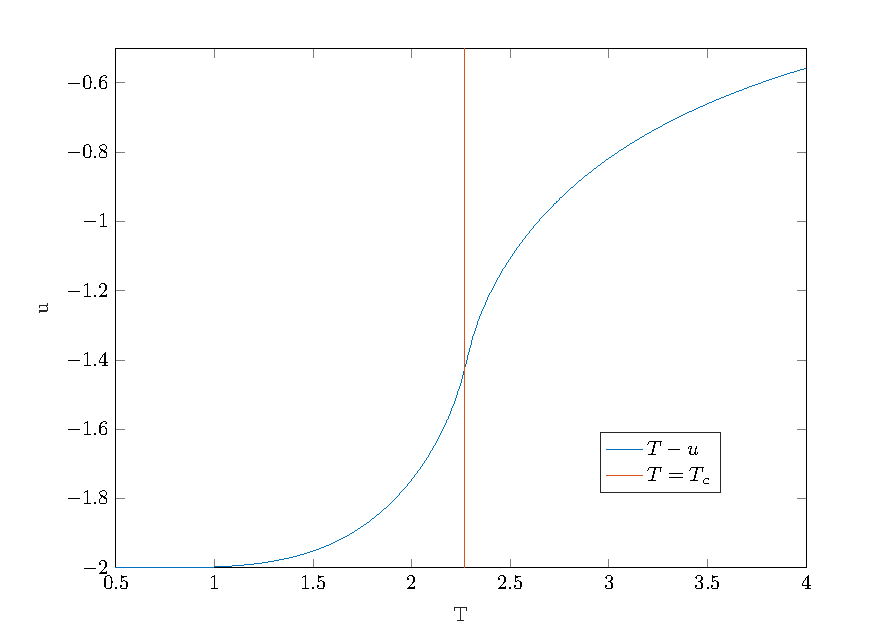
\includegraphics[width=\linewidth]{figs/Tu.pdf}
		\caption{T-u}\label{fig:Tu}
	\end{figure}
	In \Cref{pro:1}, we let \(T\) ranges in \(0.5\sim 4\) and convert \(1000000\) steps.
	In \Cref{fig:Tu} we can see as temperature become higher and higher, the value of the average Hamiltonian, \(u\), become bigger and bigger.
	That's means high temperature will supply more energy for the spins to get a state with high Hamiltonian.
	More over, we can find that the growth rate of \(u\) is highest near \(T=T_c\).
	When \(T\) is far from \(T_c\), the value of \(u\) is a virtual constant.

	In \Cref{fig:Tc} we can see that the more temperature \(T\) go near \(T_c\), the higher the specific heat is.
	\begin{figure}
		\centering
		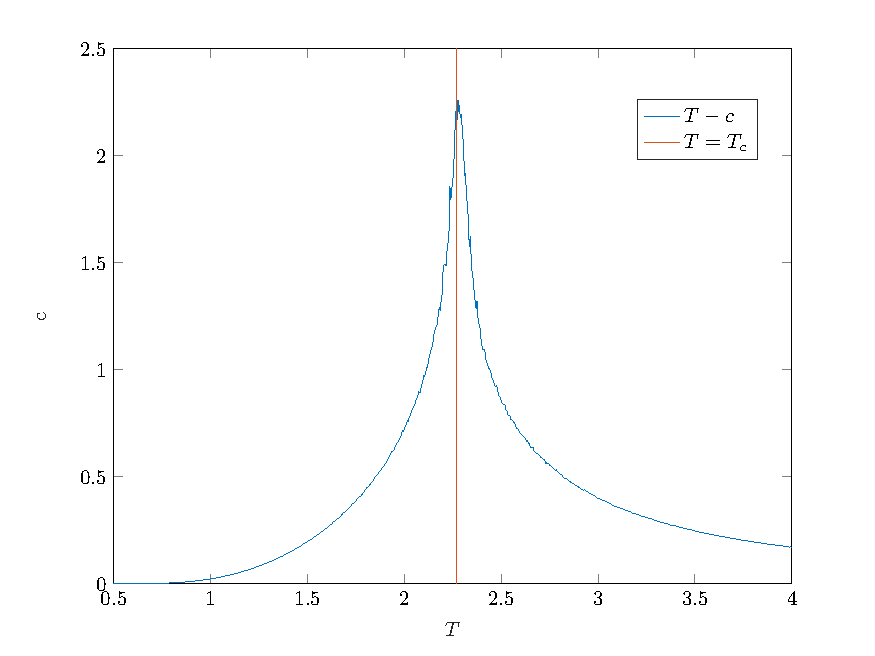
\includegraphics[width=\linewidth]{figs/Tc.pdf}
		\caption{T-c}\label{fig:Tc}
	\end{figure}
	Since the specific heat \(c\) is related to the variance of the Hamiltonian, we know that when \(T\) is near \(T_c\), the Hamiltonian will be very unstable.
	In fact, when the temperature is low, the spins will finally get into the same direction, so the Hamiltonian will be very small;
	when the temperature is high, the lattice will get very mess, every spin will get up or down randomly, so the Hamiltonian will be very big;
	when the temperature is very near to \(T_c\), the lattice will behave between them, thus the value of Hamiltonian will be big or small from time to time.
	So when \(T=T_c\) the variance of Hamiltonian will be very big.

\end{solution}

\begin{solution}
	\begin{figure}
		\centering
		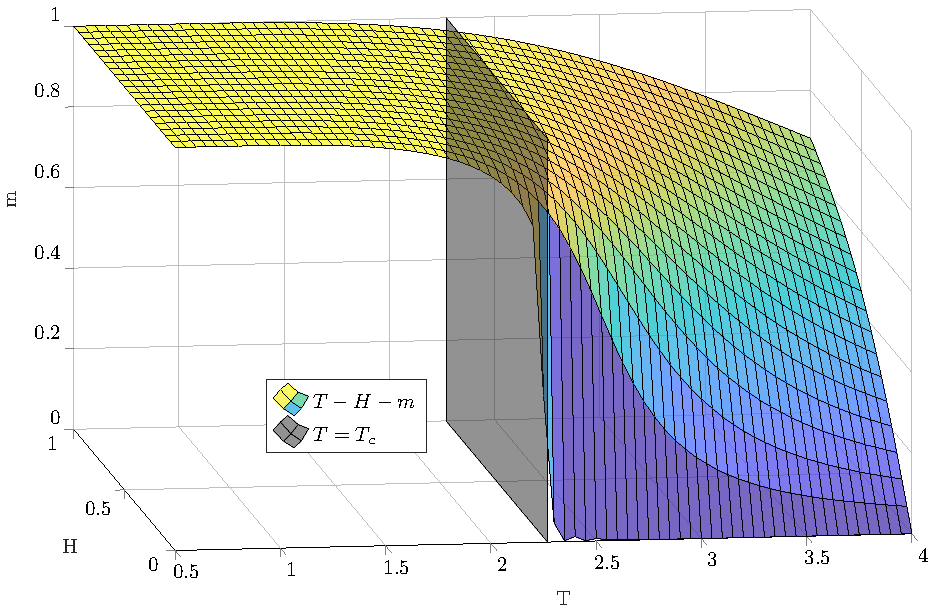
\includegraphics[width=\linewidth]{figs/THM.pdf}
		\caption{T-H-m}
		\label{fig:THM}
	\end{figure}
	We let \(T\) range from \(0.5\) to \(4\) and \(H\) range from \(0\) to \(1\) and run the program \(1000000\) steps, then compute the value of \(m\) for every pair of \(( T,H)\).
	From \Cref{fig:THM} we can find that when \(T<T_c\), the value of \(m\) will be near \(1\) not matter how small \(H\) is;
	when \(T>T_c\), the value of \(m\) just increasing follow \(H\):
	when \(H\) is small, \(m\) is near \(0\);
	when \(H\) is big, \(m\) also is big but can't reach \(1\).

	We can imagine, if this lattice is a magnet, then when the temperature is low, this magnet can easily be magnetized; when the temperature is high, this magnet can't be permanently magnetized.
\end{solution}

\section{The issues you encounter and how you overcome}
The program cost several weeks every run, but we can't let our computer work so long.
So we used our teacher's computer as server, and learned how to use ssh and sftp to work with a linux server.
\section{Possible discussion about the results and further thinking}
Ising model can not only work on a lattice but also work on a graph.
The value of \(J,H\) also can change by the index.
Using Ising on a general graph can help to solve the graph maximum cut problem.
The graph maximum cut problem is set up as following:

Let \(G\) be a weighted undirected graph.
A subset \(S\) of the vertex set \(V(G)\) of \(G\) determines a cut of the graph \(G\) into \(S\) and its complementary subset \(G\setminus S\).
The size of the cut is the sum of the weights of the edges between \(S\) and \(G\setminus S\).
A maximum cut size is at least the size of any other cut, varying \(S\).
For the Ising model without an external field on a graph \(G\), the Hamiltonian becomes the following sum over the graph edges \(E(G)\).

\begin{equation}
	H(\sigma )=-\sum _{ij\in E(G)}J_{ij}\sigma _{i}\sigma _{j}
\end{equation}

Here each vertex \(i\) of the graph is a spin site that takes a spin value \(\sigma _{i}=\pm 1\), and \(J_{ij}\) is the interaction of \(\sigma_i,\sigma_j\).
A given spin configuration \( \sigma \) partitions the set of vertices \( V(G)\) into two σ \( \sigma \)-depended subsets, those with spin up \( V^{+}\) and those with spin down \(V^{-}\).
We denote by \( \delta (V^{+})\) the \( \sigma\)-depended set of edges that connects the two complementary vertex subsets \( V^{+}\) and \( V^{-}\).
The size \( \left|\delta (V^{+})\right|\) of the cut \( \delta (V^{+})\) to bipartite the weighted undirected graph \(G\) can be defined as
\begin{equation}
	\left|\delta (V^{+})\right|={\frac {1}{2}}\sum _{ij\in \delta (V^{+})}W_{ij}
\end{equation}

where \( W_{ij}\) denotes a weight of the edge \( ij\) and the scaling \(\frac{1}{2}\) is introduced to compensate for double counting the same weights \( W_{ij}=W_{ji}\).

The identities

\begin{equation}
	\begin{aligned}H(\sigma )&=-\sum _{ij\in E(V^{+})}J_{ij}-\sum _{ij\in E(V^{-})}J_{ij}+\sum _{ij\in \delta (V^{+})}J_{ij}\\&=-\sum _{ij\in E(G)}J_{ij}+2\sum _{ij\in \delta (V^{+})}J_{ij}\end{aligned}
\end{equation}
where the total sum in the first term does not depend on \( \sigma\), imply that minimizing \( H(\sigma )\) in \( \sigma\) is equivalent to minimizing \( \sum _{ij\in \delta (V^{+})}J_{ij}\).
Defining the edge weight \( W_{ij}=-J_{ij}\) thus turns the Ising problem without an external field into a graph Max-Cut problem [4] maximizing the cut size \( \left|\delta (V^{+})\right|\), which is related to the Ising Hamiltonian as follows,

\begin{equation}
	H(\sigma )=\sum _{ij\in E(G)}W_{ij}-4\left|\delta (V^{+})\right|.
\end{equation}
%\bibliographystyle{plainnat}
%\bibliography{report}
\appendix
\begin{center}
	\large Appendix
\end{center}
\section{Vedios}
Following videos only can be played with pdf viewer supporting javascript, such as AdobeReader or Okular. Or you can play the avi file with any video player.
\begin{figure}[H]
	\centering
	\animategraphics[width=0.75\linewidth,autoplay=true,loop=true,type=pdf]{20}{./TTc/}{1}{300}
	\caption{T=Tc}
	\label{vid:Tc}
\end{figure}
\begin{figure}[H]
	\centering
	\animategraphics[width=0.75\linewidth,autoplay=true,loop=true,type=pdf]{20}{./T1/}{1}{300}
	\caption{T=1}
	\label{vid:1}
\end{figure}
\begin{figure}[H]
	\centering
	\animategraphics[width=0.75\linewidth,autoplay=true,loop=true,type=pdf]{20}{./T3/}{1}{300}
	\caption{T=3}
	\label{vid:3}
\end{figure}
\section{Codes}
\newcommand{\code}[1]{\subsection{#1}\lstinputlisting[frame=single, numbers=left, style=Matlab-editor]{codes/#1.m}}
% \lstinputlisting[frame=single, numbers=left, style=Matlab-editor]{codes/main.m}
\code{main}
\code{GenerateGrid}
\code{WhetherAccept}
\code{getDeltaEnergy}
\code{getEnergyOfGrid}
\code{pro1}
\code{pro2}
\begin{luacode*}
	tex.print([[\begin{lstlisting}]])
    for k,v in pairs(debug.getinfo(tex.print)) do 
    tex.print(string.format("%s=%s",tostring(k),tostring(v)))
    end
    tex.print(debug.getinfo(tex.print)["source"])
  tex.print([[\end{lstlisting}]])
\end{luacode*}
\end{document}                          % The required last line
